

\documentclass[10pt,journal,letterpaper,compsoc]{IEEEtran}
\usepackage{cite}
\usepackage{url}
\usepackage{times}
\usepackage{graphicx}
\usepackage{url}
\usepackage{clrscode}
\usepackage{tabularx}
\usepackage{amsmath}
\usepackage{array}
\usepackage{color}
\usepackage{balance}

\begin{document}

\title{An Implementation of the Active Contours without Edged model and the Logic Framework for Active contours on multi-channel images}

\author{Karim Ali and Sarah Nadi\\
\{karim, snadi\}@cs.uwaterloo.ca \\
David R. Cheriton School of Computer Science\\
University of Waterloo\\
}



% The paper headers
\markboth{CS870 Project Report - Active Contour without Edges}%
{Shell \MakeLowercase{\textit{et al.}}: Bare Demo of IEEEtran.cls for Computer Society Journals}


\IEEEcompsoctitleabstractindextext{%
\begin{abstract}
%\boldmath
The abstract goes here.
\end{abstract}
}

\maketitle



\section{Introduction}
Image segmentation or boundary detection is a very important problem in the area of Image Processing, and has received a lot of attention in the past. The
classical Active Contour model (or Snakes) proposed by Kass et al.~\cite{kass1988snakes} was the first model to use the idea of energy minimization to attract
a contour to the edges of the objects in an image. The Snakes model was very successful and variations of it very highly adopted later on
(E.g.~\cite{caselles1997geodesic}. Most of these models used the level set formulation for propagating fronts to evolve the curve. However, these models highly
depended on curvature motion (motion defined by the gradient of the curve) which led to poor performance in smoothed edges. To overcome these limitations, Chan
and Vese~\cite{chan2001active} propose an active contour model that does not depend on the edges (i.e the gradient) for propagating the curve to detect the
boundary of the object. Instead, they use a region-based approach based on the Mumford-Shah model~\cite{mumford1989optimal} to divide the image
into two regions: one inside the propagating curve, and one outside. The curve is at the boundary of the object if there is no difference in intensities inside
the curve as well as outside the curve.

The Active Contours without Edges model proposed by Chan and Vese (referred to as Chan-Vese model throughout the rest of this paper) was very successful in
detecting objects even in noisy or blurry images. It could also detect holes in objects which was usually a limitation in previous models. As an extension to
this work, Sandberg and Chan~\cite{sandberg2005logic} propose a logic framework (referred to as the Sandberg-Chan model throughout the rest of this
paper) that  performs logical operations on multiple images according to the curve propagation proposed in the Chan-Vese model. To achieve that, previous models
usually had two steps. They would either first segment the object in each channel separately then combine the segmented objects according to the logic operation
through bitwise operations (CITE) or they would apply logic operations to the different images then segment the resulting image (CITE). The first approach is
very costly, and the second approach requires a lot of prior knowledge about the intensities of each image. To overcome these drawbacks, the Sandberg-Chan
model is based on the idea of fitting a single contour to the object on all channels according to the logic operator, and based on regions.

In this paper, we report on our findings after implementing each of these models. We implemented both models in Matlab, and experimented with several images.
In this paper, we explain the details of our implementation as well as our results. The rest of this paper is organized as follows: Section~\ref{sec:bg} first
provides brief background about each of the two models implemented in this paper. Section~\ref{sec:implementation} then explains our implementation. In this
section, we explain how we implemented the models and any variations from the original papers. Section~\ref{sec:results} explains our evaluation criteria, and
presents the results we obtained. Section~\ref{sec:difficulties} discusses some of the difficulties we faced, and points out some BLA. Section~\ref{sec:concl}
concludes this paper by summarizing our findings.

\begin{figure*}[t]
\centering
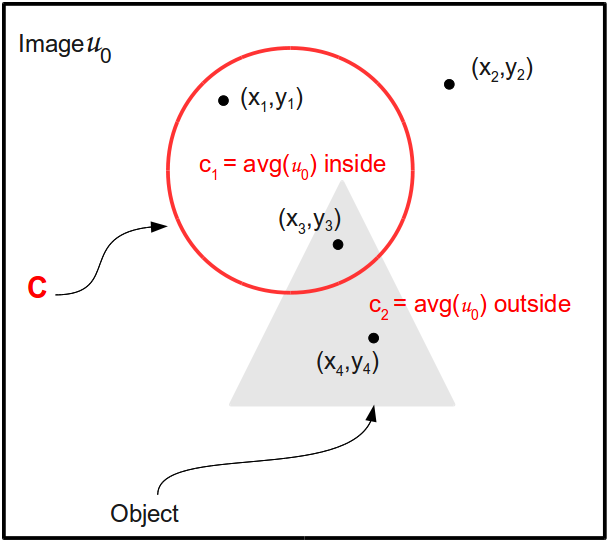
\includegraphics[width=8cm]{explaining.png}
\caption{Region Based Model}
\label{fig:region}
\end{figure*}


\section{Background}
\label{sec:bg}

\subsection{Chan-Vese Model}
\label{sec:chan-vese}

The Chan-Vese model is a region based model for detecting objects in an image. It is based on a restriction Mumford-Shah model which divides an image into
regions and represents each region by a piecewise constant (the minimal partition problem). Figure~\ref{fig:region} shows what is meant by a region based
model. The figure shows an image $u_{0}$ which has a gray triangular object in it. The red curve, C, is the initial contour used to detect this object. The
main idea behind the model is that the curve divides the image into two regions: that inside the curve and that outside. Each region is represented by a
constant, c, which is the average intensity of the image values in each region. In order for the curve to fit the object, there must be no variation of the
intensities inside the curve as well as outside. In other words, this turns into a minimization problem of the difference of intensities inside plus those
outside. For example, in the figure, the point $(x_{1},y_{1})$ will have to be outside the curve in order to minimize the difference between the points inside
the curve. Similarly, the point $(x_{4}, y_{4})$ will have to be inside the curve.

More formally, the Euler-Lagrange equation (as derived in the original paper) representing the time motion of the curve C is shown in Equation~\ref{eqn:cvpde}.

\begin{equation}
\label{eqn:cvpde}
\frac{\partial{\phi}}{\partial{t}} = \delta_{\varepsilon}(\phi)[\mu\; \mathrm{div}(\frac{\bigtriangledown \phi}{|\bigtriangledown \phi|}) - \nu -
\lambda_{1}(u_{0} - c_{1})^2 +\lambda_{2}(u_{0} - c_{2})^2] 
\end{equation}

(REST OF EQUATION HERE)

The parameter $\mu$ is a scaling parameter for the length of the curve represented in terms of curvature. The smalled $\mu$ is, the more the length of the curve
can increase without penalizing the minimization. This allows the model to detect smalled objects and holes. The larger $\mu$ is, the less freedom there is for
the curve to increase in length, and thus, it will only be able to detect larger objects. The parameter $\nu$ is also a scaling term for the area of the curve.
However, the authors do not use the area term in the Euler-Lagrange derivation, and always set $\nu$ to 0. It seems that $\mu$ is sufficient to scale the curve
according to the objects that need to be detected. Finally, $\lambda_{1}$ and $\lambda_{2}$ are weighting parameters for the forces inside the curve and
outside the curve respectively. Since we want to give both forces equal weight, the authors set $\lambda_{1} = \lambda_{2} = 1$ in all their experiments.



\subsection{Sandberg-Chan Model}
\label{sec:sandberg-chan}

\section{Implementation}
\label{sec:implementation}


\section{Experimental Results}
\label{sec:results}

\subsection{Evaluation Criteria}
\label{sec:criteria}

In order to make sure we correctly implemented the models, we had several evaluation criteria. Table~\ref{tab:criteria} summarizes these criteria, and explains
the goals of each. For the rest of this section, we proceed by presenting our experimental results in the order of these criteria starting with the simplest
cases, and incrementally challenging the model.

\begin{table*}[h!t!]
\centering
\begin{tabular}{ c | c}
\textbf{Criteria} & \textbf{Goal} \\
\hline\hline
Detecting Boundaries & Ability to correctly detect object boundaries of simple objects\\
\hline
Curve Position & Ability to correctly detect object boundaries irrespective of the initial curve position\\
\hline
Detecting Holes & Ability to detect holes in objects, and not simply stop on outside boundary\\
\hline
Blurred Images & Ability to correctly (as much as possible) detect object boundaries in blurred images\\
\hline
Noisy Images & Ability to correctly (as much as possible) detect object boundaries in noisy images\\
\hline
Parameter Settings & Ability to respond correctly to the different parameter settings
\end{tabular}
\centering
\caption{Evaluation Criteria}
\label{tab:criteria}
\end{table*}

\subsection{Criteria 1: Successfully Detecting Boundaries}

\section{Difficulties and Discussion}
\label{sec:difficulties}

\section{Conclusion}
\label{sec:concl}
The conclusion goes here.




\bibliographystyle{IEEEtran}

\bibliography{references}



% insert where needed to balance the two columns on the last page with
% biographies
%\newpage

\end{document}



